%% !TEX root = ../../handbook-physics.tex
%%!TEX TS-program = pdflatex
%%!TEX encoding = UTF-8 Unicode

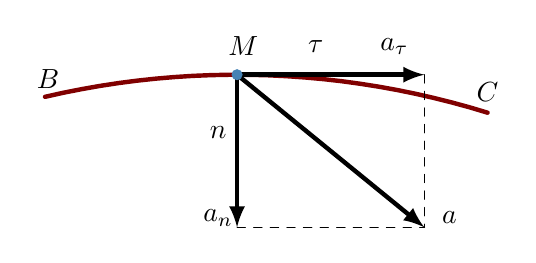
\begin{tikzpicture}[line cap=round,line join=round,scale=2]
\draw [shift={(0.,0.)},ultra thick,color=Maroon]  plot[domain=1.27:1.80,variable=\t]({1.*5.37*cos(\t r)+0.*5.37*sin(\t r)},{0.*5.37*cos(\t r)+1.*5.37*sin(\t r)});
\draw [ultra thick,-latex] (0.,5.37)-- (1.19,5.37);
\draw [ultra thick,-latex] (0.,5.37)-- (0.,4.4);
\draw [ultra thick,-latex] (0.,5.37)-- (1.19,4.4);
\draw [dashed,black] (0.,4.4)-- (1.19,4.4);
\draw [dashed,black] (1.19,5.37)-- (1.19,4.4);
%\begin{scriptsize}
\draw[color=black] (1.59,5.26) node {$C$};
\draw[color=black] (-1.20,5.34) node {$B$};
\draw[] (1,5.55) node []{$\vb{a}_{\tau}$};
\draw[] (0.5,5.55) node []{$\tau$};
\draw[] (0.04,5.55) node []{$M$};
\fill [SteelBlue] (0.,5.37) circle (1pt);
\draw[] (-0.12,4.46) node {$\vb{a}_{n}$};
\draw[] (-0.12,5.) node {$n$};
\draw[] (1.24,4.46) node [right]{$\vb{a}$};
%\end{scriptsize}
\end{tikzpicture}
